\documentclass[a4paper,12pt]{scrartcl}
\usepackage[utf8x]{inputenc}
\usepackage[T1]{fontenc} % avec T1 comme option  d'encodage c'est ben mieux, surtout pour taper du français.
%\usepackage{lmodern,textcomp} % fortement conseillé pour les pdf. On peut mettre autre chose : kpfonts, fourier,...
\usepackage[french]{babel} %Sans ça les guillemets, amarchpo
\usepackage{amsmath}
\usepackage{multicol}
\usepackage{amssymb}
\usepackage{tkz-tab}
\usepackage{exercice_sheet}

%\trait
%\section*{}
%\exo{}
%\question{}
%\subquestion{}

\date{}


% Title Page
\title{Repérage dans le plan}
 
\author{Mathématiques}

\begin{document}

\maketitle

%\tableofcontents \clearpage

\section{Repères}

\begin{definition}{Repère}
Un repère du plan est formé d'un point appelé \emph{origine} et de deux axes.

Sur chacun des axes sont définies 2 longueurs unités, une par axe (Fig. \ref{RepQuelconque}).
\end{definition}

\begin{figure}[h]
\begin{center}
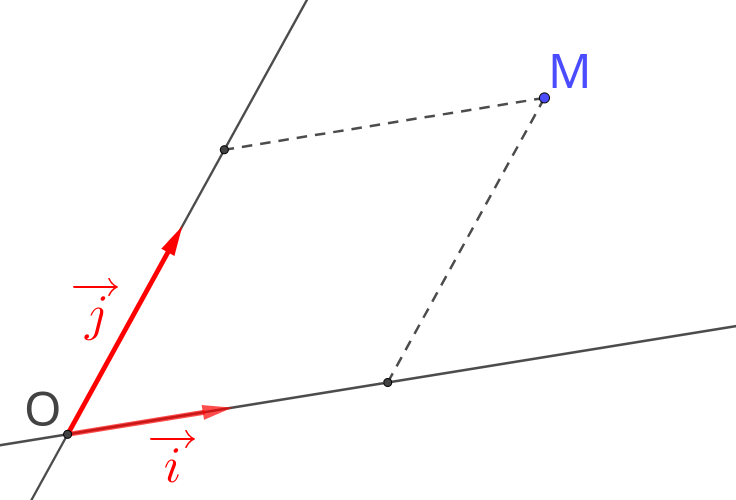
\includegraphics[width=0.6\textwidth]{pics/RepereQuelconque.png}
\end{center}
\caption{Repère quelconque}
\label{RepQuelconque}
\end{figure}

Un repère formé d'une origine $O$ et de deux vecteurs $\overrightarrow{i}$ et $\overrightarrow{j}$ est noté $\left (O;\overrightarrow{i};\overrightarrow{j}\right )$.

\subsection{Repère orthogonal}

Un repère orthogonal est un repère dont les axes sont perpendiculaires (Fig. \ref{RepOrthogonal}).

\begin{figure}[h]
\begin{center}
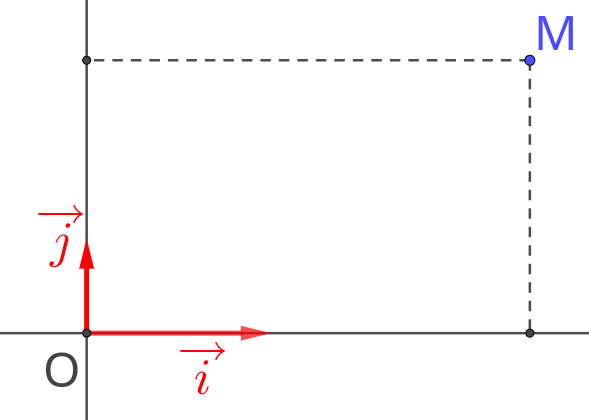
\includegraphics[width=0.4\textwidth]{pics/RepereOrthogonal.png}
\end{center}
\caption{Repère orthogonal}
\label{RepOrthogonal}
\end{figure}

De manière générale:
\begin{itemize}
\item l'axe \textbf{horizontal} est appelé axe des \textbf{abscisses} et l'abscisse est appelée $x$
\item l'axe \textbf{vertical} est appelé axe des \textbf{ordonnées} et l'ordonnée est appelée $y$
\end{itemize}


\subsection{Repère orthonormal}

Un repère orthonormal est un repère orthogonal dont l'unité de longueur en abscisses et l'unité de longueur en ordonnées sont les mêmes. 

Autrement dit, il cumule les deux propriétés: axes perpendiculaires et unités identiques sur les deux axes (Fig. \ref{RepOrthonormal}). 

\begin{figure}[h]
\begin{center}
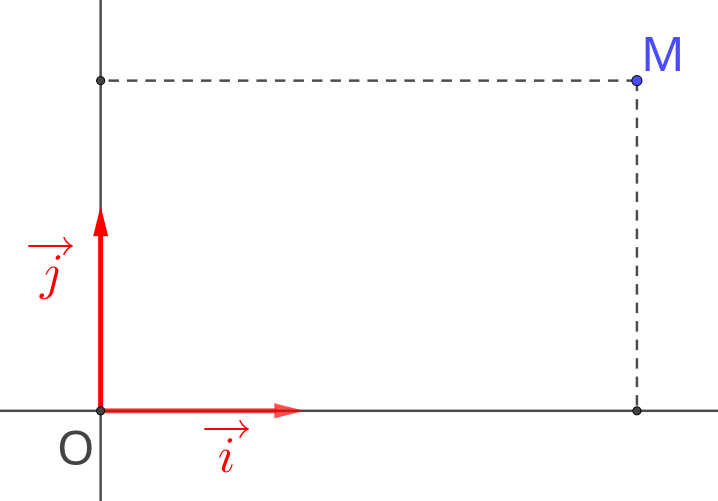
\includegraphics[width=0.4\textwidth]{pics/RepereOrthonormal.png}
\end{center}
\caption{Repère orthonormal}
\label{RepOrthonormal}
\end{figure}

\section{Coordonnées d'un point}

Dans un plan muni d'un repère $\left (O;\overrightarrow{i};\overrightarrow{j}\right )$, pour tout point $M$ il existe un unique couple de nombre réels tel que $\overrightarrow{OM} = x \overrightarrow{i} + y \overrightarrow{j}$ (Fig. \ref{JustAPoint}).

\begin{figure}[h]
\begin{center}
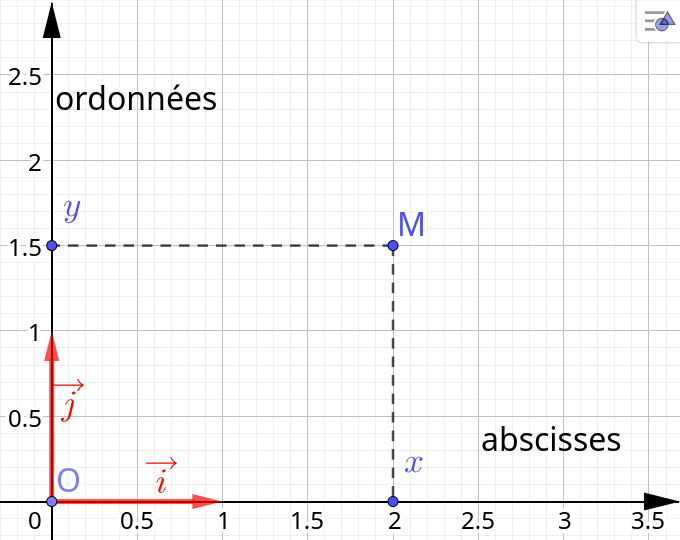
\includegraphics[width=0.45\textwidth]{pics/JustAPoint.png}
\end{center}
\caption{Point $M$ dans un repère orthogonal.}
\label{JustAPoint}
\end{figure}

Le point $M$ d'abscisse $x$ et d'ordonnée $y$ peut être noté $M(x;y)$. Sur la figure \ref{JustAPoint}, le point $M$ a pour abscisse 2 et pour ordonnée 1.5. 

\section*{Exercices}

\exo{Donner les coordonnées de chaque point:}

\begin{center}
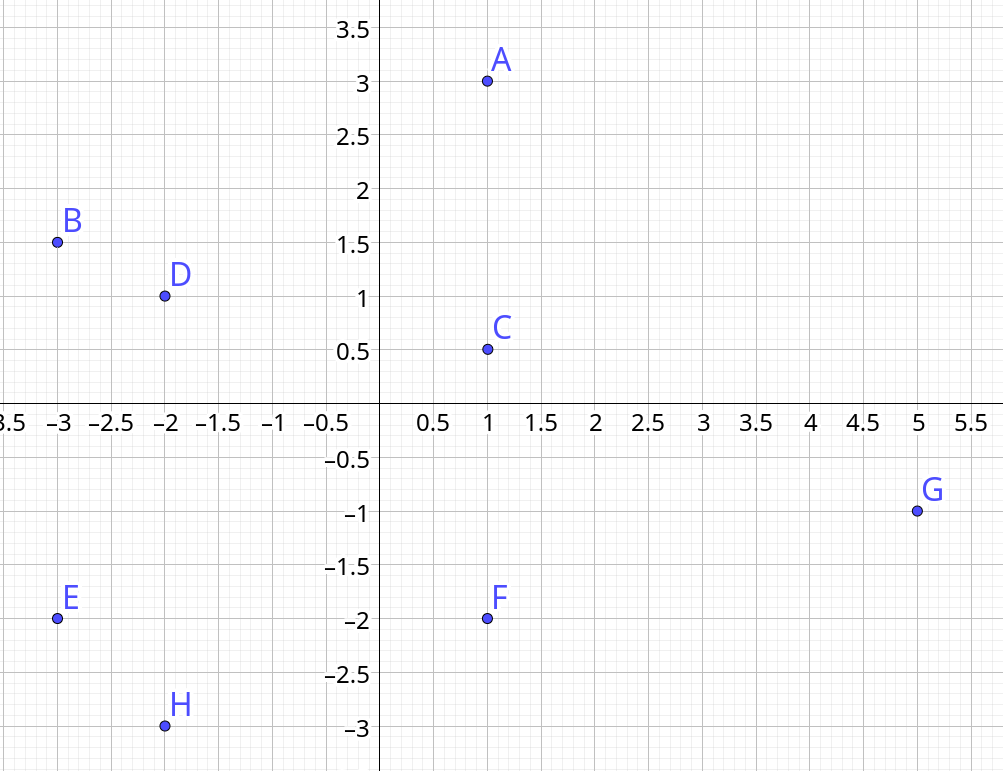
\includegraphics[width=0.8\textwidth]{pics/QuelquesPoints.png}
\end{center}

\begin{multicols}{2}
$A(\hspace{5mm};\hspace{4mm})$

\vspace{4mm}
$B(\hspace{5mm};\hspace{4mm})$

\vspace{4mm}
$C(\hspace{5mm};\hspace{4mm})$

\vspace{4mm}
$D(\hspace{5mm};\hspace{4mm})$

\vspace{4mm}
$E(\hspace{5mm};\hspace{4mm})$

\vspace{4mm}
$F(\hspace{5mm};\hspace{4mm})$

\vspace{4mm}
$G(\hspace{5mm};\hspace{4mm})$

\vspace{4mm}
$H(\hspace{5mm};\hspace{4mm})$
\end{multicols}

\exo{Placer les points suivants dans un repère en prenant 1cm pour 1 unité en abscisse et en ordonnée:}

\begin{multicols}{2}
$A(-2.5;-4.5)$

$B(6;-0.5)$

$C(-6.5;-6)$

$D(7;3.5)$

$E(-3;-5.5)$

$F(-4;-7.5)$

$G(3;6.5)$

$H(1.5;0.5)$
\end{multicols}


\end{document}
